\section{The Demo Description Language}

current version is 0.2.

\subsection{Introduction}
The Demo Description Language (DDL) is a textual description of a IPOL demo that 
allows to compile, generate a web interface, and run a demo. The description is 
written in JSON (JavaScript Object Notation) format, which is a standard format 
used in web applications. Current the JSON files are located in the 'static/JSON'
subdirectory. This language is evolving to allow a maximum number 
of demos to be described without the need to manually write HTML or Python code 
for a given demo. Each main key in the description file is described in the 
following sections:
\begin{itemize}
  \item \textit{general}: some general options;
  \item \textit{build}: everything needed to download and compile the source code;
  \item \textit{inputs}: description of the different inputs;
  \item \textit{params}: description of the parameters, for the param page;
  \item \textit{run}: commands to run the demo;
  \item \textit{config}: configuration, saving demo information;
  \item \textit{archive}: describes what is saved in archive when inputs are uploaded;
  \item \textit{results}: displaying the result page.
\end{itemize}



{\bf Note:} in JSON format, always use double quotes around keys or string 
values, not single quotes. Use can use the following link (or any other validator)
to check if your JSON code is valid: http://jsonlint.com/.
Also be carreful with commas, missing or additional commas are often the cause of
invalid JSON files.

%-------------------------------------------------------------------------------
\subsection{The \emph{general} section}
The general section describes global information about the demo.
It is a set of  (key,value) pairs, described in the following table.
Many keys are derived from the static variables of the previous 'app' Python class.\\
% 
\begin{longtable}{|>{\bf}L{\dimexpr 0.28\linewidth}|L{\dimexpr 
0.57\linewidth}|c|}
\hline
 \centering {key}     & \centering {\bf description} & {\bf req} 
\tabularnewline \hline \hline
 demo\_title         & demo title & yes\\ \hline
 input\_description  & description at the top of the input selection page, 
                      contains html as a single string or as an array of string
                      that will be concatenated and separated with spaces.
                     & yes \\ \hline
 param\_description  & description at the top of the para\-meters page,
                      contains html as a single string or as an array of string
                      that will be concatenated and separated with spaces.
                      & yes
                      \\ \hline
 xlink\_article     & defines the link to the article webpage & yes  \\ \hline
 drawmask           & boolean: if true, the demo is an mask drawing (like inpainting) demo with a 
                      single input image and mask drawing is enabled. & no \\ \hline
 drawlines          & boolean: if true, the demo is a line drawing demo with a 
                      single input image and line drawing is enabled. & no \\ \hline
 crop\_maxsize      & limit allowed crop size in both width and height, the string
                      can contain a Javascript or JQuery expression which will be evaluated & no \\ \hline
 thumbnail\_size    & set initial thumbnail size for the input selection page & no \\ \hline
 input\_condition   & sets a condition on inputs using for example the input sizes,
                      it is written as an array of 3 string, the condition,
                      the exception sent, and the error message& no \\ \hline
 show\_results\_on\-\_error & show results even if the demo returned a run-time error.
                    the demo will be able to display pertinent information & no \\ \hline
\caption{Keys for the 'general' section ({\em req} means required).}
\end{longtable}

%-------------------------------------------------------------------------------
\subsection{The \emph{build} section}

The build section contains an array of build descriptions in the form
''[ \{...\}, \{...\}, ...] ''. For each description, an archive containing the 
source code is downloaded and compiled using either 'make','cmake' or 'script' features.
It has the following information:

\subsubsection{\emph{make} type}

\begin{longtable}{|>{\bf}L{\dimexpr 0.25\linewidth}|L{\dimexpr 0.6\linewidth}|c|}
\hline
\centering {key}     & \centering {\bf description} & {\bf req} \tabularnewline 
\hline \hline
 build\_type    & make & yes \\ \hline
 url        & full url link to download the demo source code & yes \\ \hline
 srcdir     & subdirectory from the extracted archive where the source code is 
            located & yes \\ \hline
 prepare\_make & shell command used to fix compilation errors of the source code,
                since the source code is steady & no  \\ \hline
 binaries   & list of binaries and their associated paths relative to the source 
            code path. In case of 'make' build type, the first path is the compilation
            path, where the make command is called, the second path is the binary
            path. You can run make without a binary name by setting the second
            path to a directory (it should end with '/' character), then all files 
            from this directory will be copied
            to the demo binary path. If the second path is a directory, give 
            a third value corresponding to one of the files to be copied, so that
            the system can check the file timestamp to decide if rebuild is needed.
            & yes \\ \hline
 flags      & make command compilation flags & yes \\ \hline
 scripts    & list of scripts and their associated paths relative to the source 
            code path & no  \\ \hline
 post\_build & shell command to run after the build & no \\ \hline
\caption{Keys for the 'make' type.}
\end{longtable}

\paragraph{Example}:\\
\begin{lstlisting}[language=json,firstnumber=1]
"build": [ 
  {
    "build_type"    : "make",
    "url"           : "http://www.ipol.im/../phs_3.tar.gz", 
    "srcdir"        : "phs_3",
    "binaries"      : [ [".","horn_schunck_pyramidal"] ],
    "flags"         : "-j4"
  {
    "build_type"    : "make",
    "url"           : "http://www.ipol.im/../imscript_dec2011.tar.gz", 
    "srcdir"        : "imscript",
    "binaries"      : [ [".","bin/", "plambda"] ],
    "flags"          : "-j CFLAGS=-O3 IIOFLAGS='-lpng -lm'"
  }
]
\end{lstlisting}

\subsubsection{\emph{cmake} type}

\begin{longtable}{|>{\bf}L{\dimexpr 0.25\linewidth}|L{\dimexpr 0.6\linewidth}|c|}
\hline
\centering {key}     & \centering {\bf description} & {\bf req} \tabularnewline 
\hline \hline
 build\_type  & cmake & yes \\ \hline
 url          & same as make type & yes \\ \hline
 srcdir       & same as make type & yes \\ \hline
 prepare\_cmake & shell command used to fix compilation errors of the source code,
                since the source code is steady & no  \\ \hline
 cmake\_flags  & cmake flags for configuration ('Release' build type is 
                automatically set) & no  \\ \hline
 binaries     & same as make type & yes \\ \hline
 flags        & same as make type & yes \\ \hline
 scripts      & same as make type & no  \\ \hline
 post\_build  & same as make type & no \\ \hline
\caption{Keys for the 'cmake' type.}
\end{longtable}

\paragraph{Example}:\\
\begin{lstlisting}[language=json,firstnumber=1]
"build": [ { 
  "build_type" : "cmake",
  "url"        : "http://www.ipol.im/xxx/ldm_q1p.zip", 
  "srcdir"     : ".",
  "binaries"   : [ [".","lens_distortion_correction"] ],
  "flags"      : "OMP=1 -j4" } ]
\end{lstlisting}

\subsubsection{\emph{script} type}

\begin{longtable}{|>{\bf}L{\dimexpr 0.25\linewidth}|L{\dimexpr 0.6\linewidth}|c|}
\hline
\centering {key}     & \centering {\bf description} & {\bf req} \tabularnewline 
\hline \hline
 build\_type  & script & yes \\ \hline
 url          & same as make type & yes \\ \hline
 srcdir       & same as make type & yes \\ \hline
 scripts      & same as make type & no  \\ \hline
\caption{Keys for the 'script' type.}
\end{longtable}

\paragraph{Example}:\\
\begin{lstlisting}[language=json,firstnumber=1]
"build": [ { 
    "build_type": "script",
    "url": "http://151.80.24.28:8080/DemoSource/1000003/demo_scripts.tgz",
    "srcdir": "demo_scripts",
    "scripts": [ [ ".", "write_line_parameters.py" ] ]
  }
\end{lstlisting}


%-------------------------------------------------------------------------------
\subsection{The \emph{inputs} section}
The inputs section describes the set of input data of the algorithm (images, 
videos, flows, etc..).

\subsubsection{\emph{image} type}

\begin{longtable}{|>{\bf}L{\dimexpr 0.17\linewidth}|L{\dimexpr 0.68\linewidth}|c|}
\hline
\centering {key}     & \centering {\bf description} & {\bf req} \tabularnewline 
\hline \hline
 type         & image & yes \\ \hline
 description  & Short name or description of the input, it will used to display 
the input as the label inside the 'gallery' html display & yes \\ \hline
 max\_pixels   &  sets the maximal number of pixels of the input image, 
bigger images will be downsized, if 0 no resizing is done. The resizing as 
defined in the image class uses python PIL resizing with 'antialias' option. 
Input can be a number or a string that will be evaluated in Javascript.  & .. \\ \hline
 max\_weight   & max size (in bytes) of an input file, prevents uploading 
bigger files. Input can be a number or a string that will be evaluated in Javascript. & .. \\ \hline
 dtype        & input image expected data type, used as parameter of 
image.convert() method. Possible values are '1x8i' and '3x8i' which are 
converted respectively to 'L' and 'RGB' for PIL. & .. \\ \hline
 ext          & input image expected extention (ie. file format) & .. \\ \hline
\caption{Keys for the 'image' type.}
\end{longtable}

\subsubsection{\emph{flow} type}

\ToDo{[Karl]: explain how to assiocate an image to represent the flow. }


\begin{longtable}{|>{\bf}L{\dimexpr 0.17\linewidth}|L{\dimexpr 0.68\linewidth}|c|}
\hline
\centering {key}     & \centering {\bf description} & {\bf req} \tabularnewline 
\hline \hline
 type             & flow & yes \\ \hline
 description      & same as image & yes \\ \hline
 ext              & same as image & yes \\ \hline
 required         & boolean: tells if the flow is required for the algorithm
or optional, default is optional. For example, the ground truth may be optional.& no \\ \hline
\caption{Keys for the 'flow' type.}
\end{longtable}


%-------------------------------------------------------------------------------
\subsection{The \emph{params} section}
The params section describes the set of parameters needed by a demo, their 
constraints and their visual appearance. It is defined as an array of sets, 
where each set contains (key,value) pairs.


\subsubsection{ \emph{range} type}

The values of the range type are stored as numbers, so no double quotes are 
required around the values. The default value is stored with the 'values' field.

\begin{longtable}{|>{\bf}L{\dimexpr 0.15\linewidth}|L{\dimexpr 
0.7\linewidth}|c|}
\hline
 \centering {key}     & \centering {\bf description} & {\bf req} 
\tabularnewline \hline \hline
 type  & range       & yes \\ \hline
 visible  & Javascript/JQuery boolean expression evaluted in the context defined 
              in \ref{sec:JavascriptEvalParams} that can hide the parameter if
            evaluated to false (if undefined the parameter is visible)& no \\ \hline
 id     & parameter name in lowercase letters  & yes \\ \hline
 label  & name and/or description of the parameter, appears on the left side. & yes
                      \\ \hline
 comments & description of the parameter, appears on the right side. & no
                      \\ \hline
 values & set min,max,step and default values using the following key/value 
scheme \{ 'min':val, 'max':val, 'step':val, 'default':val \} & yes
                      \\ \hline
\caption{Keys for the 'range' type.}
\end{longtable}

\subsubsection{ \emph{range\_scientific} type}

The values of the range type are stored as numbers, so no double quotes are 
required around the values. The default value is stored with the 'values' field.
The 'range\_scientific' type differs from the 'range' type because it displays
the values in scientific notation with mantissa and exponent, the 'digits' parameter
sets the number of digits after the decimal points for the mantissa, the slider
will also to change each digit.

\begin{longtable}{|>{\bf}L{\dimexpr 0.15\linewidth}|L{\dimexpr 
0.7\linewidth}|c|}
\hline
 \centering {key}     & \centering {\bf description} & {\bf req} 
\tabularnewline \hline \hline
 type  & range\_scientific       & yes \\ \hline
 visible  & Javascript/JQuery boolean expression evaluted in the context defined 
              in \ref{sec:JavascriptEvalParams} that can hide the parameter if
            evaluated to false (if undefined the parameter is visible)& no \\ \hline
 id     & parameter name in lowercase letters  & yes \\ \hline
 label  & name and/or description of the parameter, appears on the left side. & yes
                      \\ \hline
 comments & description of the parameter, appears on the right side. & no
                      \\ \hline
 values & set min,max,step and default values using the following key/value 
scheme \{ 'min':val, 'max':val, 'digits':val, 'default':val \} & yes
                      \\ \hline
\caption{Keys for the 'range\_scientific' type.}
\end{longtable}


\subsubsection{ \emph{selection\_collapsed} type}

The values of the selection are stored as strings, so we map each label with a 
string value. The default value is stored in a separate field.

\begin{longtable}{|>{\bf}L{\dimexpr 0.25\linewidth}|L{\dimexpr 
0.6\linewidth}|c|}
\hline
 \centering {key}     & \centering {\bf description} & {\bf req} 
\tabularnewline \hline \hline
 type  & selection\_collapsed    & yes \\ \hline
 visible  & Javascript/JQuery boolean expression evaluted in the context defined 
              in \ref{sec:JavascriptEvalParams} that can hide the parameter if
            evaluated to false (if undefined the parameter is visible)& no \\ \hline
 id     & parameter name in lowercase letters & yes \\ \hline
 label  & name and/or description of the parameter, appears on the left side. & yes
                      \\ \hline
 comments & description of the parameter, appears on the right side. & no
                      \\ \hline
 values & set of (key,value) pairs, where the key is the displayed text and the 
value a string representing the corresponding value, for example \{ 
'black':'0', '1\%':'0.01' \} & yes
                      \\ \hline
 default\_value & defines the default value for this parameter, should be one 
the values defined in 'values'. & yes \\ \hline
\caption{Keys for the 'selection\_collapsed' type.}
\end{longtable}

\subsubsection{ \emph{selection\_radio} type}

The values of the selection are stored as strings, so we map each label with a 
string value. The default value is stored in a separate field.
This type is similar to the selection collapsed type, but display the different
options using radio buttons.

\begin{longtable}{|>{\bf}L{\dimexpr 0.25\linewidth}|L{\dimexpr 
0.6\linewidth}|c|}
\hline
 \centering {key}     & \centering {\bf description} & {\bf req} 
\tabularnewline \hline \hline
 type     & selection\_radio    & yes \\ \hline
 visible  & Javascript/JQuery boolean expression evaluted in the context defined 
              in \ref{sec:JavascriptEvalParams} that can hide the parameter if
            evaluated to false (if undefined the parameter is visible)& no \\ \hline
 id       & parameter name in lowercase letters & yes \\ \hline
 label  & name and/or description of the parameter, appears on the left side. & yes
                      \\ \hline
 comments & description of the parameter, appears on the right side. & no
                      \\ \hline
 vertical & boolean, if true use vertical display, otherwise use horizontal
            display (default=false) & no \\ \hline
 values   & set of (key,value) pairs, where the key is the displayed text and the 
value a string representing the corresponding value, for example \{ 
'black':'0', '1\%':'0.01' \} & yes
                      \\ \hline
 default\_value & defines the default value for this parameter, should be one 
the values defined in 'values'. & yes \\ \hline
\caption{Keys for the 'selection\_radio' type.}
\end{longtable}

\subsubsection{ \emph{label} type}

The label  can be used as a title to separate groups of parameters.

\begin{longtable}{|>{\bf}L{\dimexpr 0.27\linewidth}|L{\dimexpr 
0.58\linewidth}|c|}
\hline
 \centering {key}     & \centering {\bf description} & {\bf req} 
\tabularnewline \hline \hline
 type  & label       & yes \\ \hline
 visible  & Javascript/JQuery boolean expression evaluted in the context defined 
              in \ref{sec:JavascriptEvalParams} that can hide the parameter if
            evaluated to false (if undefined the parameter is visible)& no \\ \hline
 label & html text to display, as a single string or as an array of strings& yes
                      \\ \hline
\caption{Common keys for the 'label' type.}
\end{longtable}


\subsubsection{ \emph{readonly} type}

\begin{longtable}{|>{\bf}L{\dimexpr 0.27\linewidth}|L{\dimexpr 
0.58\linewidth}|c|}
\hline
 \centering {key}     & \centering {\bf description} & {\bf req} 
\tabularnewline \hline \hline
 type  & readonly    & yes \\ \hline
 visible  & Javascript/JQuery boolean expression evaluted in the context defined 
              in \ref{sec:JavascriptEvalParams} that can hide the parameter if
            evaluated to false (if undefined the parameter is visible)& no \\ \hline
 label & description of the parameter & yes \\ \hline
 id         & parameter name in lowercase letters  & yes \\ \hline
 value\_expr & Javascript/JQuery expression used to compute the parameter value, defined as an
              array of strings that will be concatenated to a single string.
            & yes \\ \hline
\caption{Common keys for the 'readonly' type.}
\end{longtable}

\subsubsection{ \emph{checkbox} type}

\begin{longtable}{|>{\bf}L{\dimexpr 0.27\linewidth}|L{\dimexpr 
0.58\linewidth}|c|}
\hline
 \centering {key}     & \centering {\bf description} & {\bf req} 
\tabularnewline \hline \hline
 type  & checkbox  & yes \\ \hline
 visible  & Javascript/JQuery boolean expression evaluted in the context defined 
              in \ref{sec:JavascriptEvalParams} that can hide the parameter if
            evaluated to false (if undefined the parameter is visible)& no \\ \hline
 label  & name and/or description of the parameter, appears on the left side. & yes
                      \\ \hline
 comments & description of the parameter, appears on the right side. & no
                      \\ \hline
 id         & parameter name in lowercase letters  & yes \\ \hline
 default\_value & boolean: True for checked & \\ \hline
\caption{Common keys for the 'checkbox' type.}
\end{longtable}

\subsubsection{ \emph{checkboxes} type}

\begin{longtable}{|>{\bf}L{\dimexpr 0.27\linewidth}|L{\dimexpr 
0.58\linewidth}|c|}
\hline
 \centering {key}     & \centering {\bf description} & {\bf req} 
\tabularnewline \hline \hline
 type  & checkboxes   & yes \\ \hline
 visible  & Javascript/JQuery boolean expression evaluted in the context defined 
              in \ref{sec:JavascriptEvalParams} that can hide the parameter if
            evaluated to false (if undefined the parameter is visible)& no \\ \hline
 label  & name and/or description of the parameter, appears on the left side. & yes
                      \\ \hline
 comments & description of the parameter, appears on the right side. & no
                      \\ \hline
 id         & parameter name in lowercase letters  & yes \\ \hline
 values     & list of dictionaries: [ {key:value, ...}, ... ]
            where key is the checkbox id and value is the text associated
            & yes \\ \hline
 default     & list of checkboxes that are checked by default  & yes \\ \hline
\caption{Common keys for the 'checkboxes' type.}
\end{longtable}


%-------------------------------------------------------------------------------
\subsection{The \emph{params\_layout} section}

The default layout of parameters is to stack them together within an 'HTML field'
entitle 'Parameters:'. However, if a demo needs to group together some parameters,
it can use a specific params\_layout section that contains an array of
sets of parameters, where each set is defined by an array containing the group 
title as the first element and the list of parameters ids as the second element,
where the parameters ids are their position in the params section (starting at 0).

\paragraph{Examples}:\\
\begin{lstlisting}[language=json,firstnumber=1]
  "params_layout": [
        [ "General parameters:",          [ 0,1]  ],
        [ "Sampled Gaussian kernel",      [2]     ],
        [ "Lindeberg's smoothing method", [3]     ]
    ],
\end{lstlisting}

%-------------------------------------------------------------------------------
\subsection{The \emph{run} section}

The 'run' section contains an array of elements, where each element can be 
a string or another array of strings:
\begin{itemize}
\item if the element is a string starting with '\#', it is considered as a comment.
\item if the element is a string, it can be a command to run from the system (shell, 
python script or demo binary) or a python code to evaluate if the string
starts with "python:",
\item if the element is an array of strings, the first string is a python
condition, if this condition is fulfilled, the remaining commands will be
executed.
\end{itemize}
In the command line, you can use \$param\_id to evaluate a 
python expression that can contain the parameter ids,
and '\textgreater output\_file' (without space between '\textgreater' and the 
filename) to redirect the standard output to a given file, save in the current 
working directory. 
If you also want to redirect the standard errors to the same file, use can add 
'2\textgreater\&1' as another argument. However, pipelines are not allowed 
('|' character).
Python scripts from the PythonTools directory can be used in commands: currently
'count\_lines.py' and 'image\_histogram.py'.
If you want to access specific demo data copied in the binary directory, use must
use the variable 'demodata', for example "cp \$\{demodata\}/\-pattern\-\_noise.pgm .".


\paragraph{Examples}:\\
\begin{lstlisting}[language=json,firstnumber=1]
"run": [
  "#--- comment ---"
  "nlmeans  input_0.sel.png $sigma input_1.png output_1.png",
  "img_diff input_0.sel.png input_1.png $sigma output_2.png",
  "img_mse  input_0.sel.png output_1.png >stdout.txt 2>&1"
]
\end{lstlisting}

In this example, the last command adds a new parameters using self.algo\_params,
this parameter will be saved in the config files. It is also possible to add 
or change info and meta sections using self.algo\_info and self.algo\_meta.
\begin{lstlisting}[language=json,firstnumber=1]
  "run": [ 
    "mosaic     -p $pattern input_0.sel.png mosaiced.png ",
    "python:sizeX=x1-x0;sizeY=y1-y0",
    "python:zoom_factor=max(1, int(math.ceil(200.0/min(sizeX, sizeX))))",
    "python:sizeX=sizeX*zoom_factor;sizeY=sizeY*zoom_factor",
    "convert -filter point -resize ${sizeX}x${sizeY} input_0.sel.png    input_0.sel_zoom.png",
    "python:self.algo_params['zoom_factor']=zoom_factor"
  ]
\end{lstlisting}

A more complex example taken from demo 70:
\begin{lstlisting}[language=json,firstnumber=1]
  "run": [ 
      "convert input_0.sel.png inputNG.pgm",
      [ "threshold_type=='manual'", 
          "pgm2freeman -min_size $min_c -image inputNG.pgm -outputSDPAll -maxThreshold $tmax -minThreshold $tmin >inputPolygon.txt 2>algoLog.txt"
      ],
      [ "threshold_type=='auto'",   
          "pgm2freeman -min_size $min_c -image inputNG.pgm -outputSDPAll >inputPolygon.txt 2>algoLog.txt",
          "python:fInfo = open(self.work_dir+'algoLog.txt', 'r')",
          "python:lines = fInfo.readlines()",
          "python:line_cases = lines[0].replace(')', ' ').split();",
          "python:tmax = int(line_cases[17])"
      ],
      "python:contoursList = open (self.work_dir+'inputPolygon1.txt', 'w')",
      ...
  ]
\end{lstlisting}
 

%-------------------------------------------------------------------------------
\subsection{The \emph{config} section}

The config section is optional, it allows creating new (key,value) pairs in the 
configuration file based on text files obtained during the execution. This 
new information can then be used in the archive section.

\begin{longtable}{|>{\bf}L{\dimexpr 0.25\linewidth}|L{\dimexpr 0.6\linewidth}|c|}
\hline
\centering {key}     & \centering {\bf description} & {\bf req} \tabularnewline 
\hline \hline
 info\_from\_file    & it contains a list of (key,value) pairs where the key is
            the new information id to create (in lowercase letters) and the
            value is the corresponding text file that contains its contents & no \\ \hline
\caption{keys for the 'config' section.}
\end{longtable}

\paragraph{Example}:\\
\begin{lstlisting}[language=json,firstnumber=1]
"config":
  {
    "info_from_file": {  "homography_1" : "output_0.txt",
                          "homography_2" : "output_1.txt"
                      }
  }
\end{lstlisting}

%-------------------------------------------------------------------------------
\subsection{The \emph{archive} section}


\begin{longtable}{|>{\bf}L{\dimexpr 0.25\linewidth}|L{\dimexpr 0.6\linewidth}|c|}
\hline
\centering {key}     & \centering {\bf description} & {\bf req} \tabularnewline 
\hline \hline
 files    & (key,value) pairs where key is the file to archive and value is 
            the associated text information & no \\ \hline
 compressed\_\-files   & compressed files to add in the same format 
as files & no \\ \hline
 params  & list of parameters to archive & no \\ \hline
 info    & info variables to archive in the form of pairs variable:label & no \\ \hline
\caption{Keys for the 'text\_file' type.}
\end{longtable}


\paragraph{Example}:\\
\begin{lstlisting}[language=json,firstnumber=1]
"archive":
  {
    "files" : 
      { "input_0.png"                 : "input image",
        "primitives.txt"              : "Primitives"  },
    "params" :  
      [ "high_threshold_canny", 
        "initial_distortion_parameter", 
        "angle_point_orientation_max_difference" ],
    "info"   : { "run_time": "run time" }
  }
\end{lstlisting}

%-------------------------------------------------------------------------------
\subsection{The \emph{results} section}


The results section also contains an array of sets, where each set contains 
(key/value) pairs describing one type of output from the algorithm. There are 
displayed sequentially one below the other, a part from warnings that are 
displayed at the top of the page. The currently available types are described 
below. At the top of the results page, the processing time is displayed and the 
user is proposed to run the demo again with different input or parameters.


%------ gallery  ------
\subsubsection{ \emph{gallery} type}

The gallery type uses the gallery class to display images. Its parameters are:

\begin{longtable}{|>{\bf}L{\dimexpr 0.15\linewidth}|L{\dimexpr 0.7\linewidth}|c|}
\hline
 \centering {key}     & \centering {\bf description} & {\bf req} 
\tabularnewline \hline \hline
 type       & gallery  & yes \\ \hline
 visible    & Javascript/JQuery boolean expression evaluted in the context 
              defined in \ref{sec:JavascriptEval}, that can hide the result if
              evaluated to false (if undefined the result is visible)& no \\ \hline
 label      & html label for the gallery, can be either a single string or 
             a list of string that will be concatenated with whitespace character
              in between. & yes \\ \hline
 contents   & pairs of label:imagecontents information, where imagecontents can 
              have three different forms: a filename, an array of filenames, or
              a list of title:filename pairs. 
              If an image filename does succeed in loading,
              the image will be removed from the gallery. 
              You can also add a condition evaluated in Javascript,
              in the current context to enable or disable the pair display:
              using a label string of the form "condition?label".
            & yes \\ \hline
 options    & You can specify options for the ImageGallery object. Currently
              'minwidth' and 'minheight' (in pixels) options are available to force
              miminal size of image display. Default values are 300 for both.& no \\ \hline
\caption{Keys for the 'gallery' type.}
\end{longtable}

\paragraph{Examples}:\\
Standard example, using single filename strings.
\begin{lstlisting}[language=json,firstnumber=1]
  { "type"          : "gallery",
    "label"         : "<h2>Resulting images</h2>",
    "contents"      : { 
      "Input"     : "input_0.sel.png", 
      "Output"    : "output.png"
    },
    "options"     : { "minheight" : 400 }
  },
\end{lstlisting}
The use of '?' in the label "meta.hastruth?Ground truth" will condition the 
display of "t.ipol.png" image based on the boolean variable meta.hastruth.
\begin{lstlisting}[language=json,firstnumber=1]
  { "type"    : "gallery",
    "label"   : "<h2>Images</h2>",
    "contents": 
      {
        "Optical flow "              : "stuff_phs.ipol.png", 
        "meta.hastruth?Ground truth" : "t.ipol.png",
      }
   },
\end{lstlisting}
The use of pairs title:filename in the contents will display a HTML table
for each tab (here "DFT" and "DCT") with images and their associated titles.
\begin{lstlisting}[language=json,firstnumber=1]
  { "type"          : "gallery",
    "label"         : "<h2>Gaussian filter results</h2>",
    "contents"      : { 
      "DFT":
        { "1 iteration" :"dft_direct.png", 
          "N iterations":"dft_iter.png", 
          "difference"  :"dft_diff.png" }, 
      "DCT":                     
        { "1 iteration" :"dct_direct.png", 
          "N iterations":"dct_iter.png",
          "difference"  :"dct_diff.png" }
    }
  },
\end{lstlisting}
The use of string array in the contents will display HTML table without associated
titles.
\begin{lstlisting}[language=json,firstnumber=1]
  { "type"          : "gallery",
    "label"         : "<p>The following images were resized...<p>",
    "contents"      : { 
      "zoomed-out"  : [ "ipol_imgW.png", "palette1.png" ],
      "zoomed-in"   : [ "ipol_imgC.png", "palette1.png" ],
      "residue"     : [ "ipol_diff.png", "palette2.png" ],
      "mask"        : [ "ipol_mask.png", "palette1.png" ]
    }
  },
\end{lstlisting}


%------ file_download  ------
\subsubsection{ \emph{file\_download} type}

\begin{longtable}{|>{\bf}L{\dimexpr 0.15\linewidth}|L{\dimexpr 0.7\linewidth}|c|}
\hline
\centering {key}     & \centering {\bf description} & {\bf req} \tabularnewline 
\hline \hline
 type      & file\_download  & yes \\ \hline
 visible   & Javascript/JQuery boolean expression evaluted in the context defined 
              in \ref{sec:JavascriptEval}, that can hide the result if
             evaluated to false (if undefined the result is visible)& no \\ \hline
 repeat    & range expression (evaluated in Javascript):
              will create a loop in the form idx=0..range-1 & no \\ \hline
 label     & html title associated to the file download. In case of repeat, 
            evaluated as an expression with idx variable, otherwise, can be evaluated
            if it starts with single quote.& yes \\ \hline
 contents  & either a single string of the filename to download, or a list
              of label:filename pairs for files to download. In case of repeat, 
            evaluated as an expression with idx variable. & yes \\ \hline
\caption{Keys for the 'file\_download' type.}
\end{longtable}

\paragraph{Examples}:\\
\begin{lstlisting}[language=json,firstnumber=1]
  { "type"     : "file_download", 
    "label"    : "Download Hough result",
    "contents" : "output_hough.png" },
\end{lstlisting}

\begin{lstlisting}[language=json,firstnumber=1]
  {
    "type"          : "file_download", 
    "label"         : "<h3>Download computed optical flow:</h3>",
    "contents"      : { "tiff": "stuff_tvl1.tiff", 
                        "flo" : "stuff_tvl1.flo",
                        "uv"  : "stuff_tvl1.uv" }  },
\end{lstlisting}
Example using 'repeat':
\begin{lstlisting}[language=json,firstnumber=1]
  { "type"          : "file_download", 
    "repeat"        : "params.scales",
    "label"         : "'Download the estimations obtained at scale '+idx",
    "contents"      : "'estimation_s'+idx+'.txt'" }
\end{lstlisting}

%------ html_text  ------
\subsubsection{ \emph{html\_text} type}

\begin{longtable}{|>{\bf}L{\dimexpr 0.15\linewidth}|L{\dimexpr 0.7\linewidth}|c|}
\hline
\centering {key}     & \centering {\bf description} & {\bf req} \tabularnewline 
\hline \hline
 type      & html\_text  & yes \\ \hline
 visible   & Javascript/JQuery boolean expression evaluted in the context 
             defined in \ref{sec:JavascriptEval}, that can hide the result if
             evaluated to false (if undefined the result is visible)& no \\ \hline
 contents  & array of strings, that will be concatenated to form the html 
             content. This content can contain Javascript/JQuery expression if it starts
            with a single quote. & yes \\ \hline
\caption{Keys for the 'html\_text' type.}
\end{longtable}

\paragraph{Example}:\\
\begin{lstlisting}[language=json,firstnumber=1]
  { "type"          : "html_text", 
    "contents"      : [
      "'<p style=\"font-size:85%\">",
        "* &ldquo;Exact&rdquo; is computed with FIR, ",
        "DCT for &sigma;&nbsp;&gt;&nbsp;2 ",
        "(using '+params.sigma<=2?'FIR':'DCT'+",
      "'</p>'" ] },
\end{lstlisting}


%------------ text_file --------------------------
\subsubsection{ \emph{text\_file} type}

\begin{longtable}{|>{\bf}L{\dimexpr 0.15\linewidth}|L{\dimexpr 0.7\linewidth}|c|}
\hline
\centering {key}     & \centering {\bf description} & {\bf req} \tabularnewline 
\hline \hline
 type      & text\_file  & yes \\ \hline
 visible   & Javascript/JQuery boolean expression evaluted in the context 
              defined in \ref{sec:JavascriptEval}, that can hide the result if
             evaluated to false (if undefined the result is visible)& no \\ \hline
 label     & HTML label & yes \\ \hline
 contents  & text filename to display & yes \\ \hline
 style     & associated CSS style & yes \\ \hline
\caption{Keys for the 'text\_file' type.}
\end{longtable}

\paragraph{Example}:\\
\begin{lstlisting}[language=json,firstnumber=1]
  { "type"          : "text_file", 
    "label"         : "<h2>Output<h2>",
    "contents"      : "stdout.txt",
    "style"         : "width:40em;height:16em;background-color:#eee" }
\end{lstlisting}

%------ warning  ------
\subsubsection{ \emph{warning} type}

\begin{longtable}{|>{\bf}L{\dimexpr 0.15\linewidth}|L{\dimexpr 
0.7\linewidth}|c|}
\hline
 \centering {key}     & \centering {\bf description} & {\bf req} 
\tabularnewline \hline \hline
 type      & warning  & yes \\ \hline
 visible   & Javascript/JQuery boolean expression evaluted in the context 
            defined in \ref{sec:JavascriptEval}, that can hide the result if
             evaluated to false (if undefined the result is visible)& no \\ \hline
 contents  & displayed text, can contain both HTML tags and Javascript/JQuery code.
expressions of the form '\{\{expression\}\}'. & \\ \hline
\caption{Keys for the 'warning' type.}
\end{longtable}
\paragraph{Example}:\\
\begin{lstlisting}[language=json,firstnumber=1]
{ "type":"warning", 
  "condition":"sizeX * sizeY < X",
  "contents":"'Needs X pixels ('+sizeX *sizeY+' given)<br/>'"},
\end{lstlisting}


%------ repeat_gallery  ------
\subsubsection{ \emph{repeat\_gallery} type}
The repeat\_gallery type is design to display a gallery with a number of images 
that depend on a parameter, for example the number of scales used by the 
algorithm.

\begin{longtable}{|>{\bf}L{\dimexpr 0.15\linewidth}|L{\dimexpr 0.7\linewidth}|c|}
\hline
\centering {key}     & \centering {\bf description} & {\bf req} \tabularnewline 
\hline \hline
 type       & repeat\_gallery  & yes \\ \hline
 visible    & Javascript/JQuery boolean expression evaluted in the context 
              defined in \ref{sec:JavascriptEval}, that can hide the result if
              evaluated to false (if undefined the result is visible)& no \\ \hline
 label      & html label for the gallery, can be either a single string or 
             a list of string that will be concatenated with whitespace character
              in between.& yes \\ \hline
 repeat     & range expression (evaluated in Javascript):
              will create a loop in the form idx=0..range-1 & yes \\ \hline
 contents   & an array where the first element is a string representing the label
              and that can contain Javascript/JQuery expression using the index idx, and
              the second element is either a string or an array of strings
              representing the image filenames to display. & yes \\ \hline
 options    & see 'gallery' type. & yes \\ \hline
\caption{Keys for the 'repeat\_gallery' type.}
\end{longtable}

\paragraph{Examples}:\\
\begin{lstlisting}[language=json,firstnumber=1]
  { "type"     : "repeat_gallery",
    "repeat"   : "params.scales",
    "label"    : "<h2> Noise Curves </h2>",
    "contents" : [ "'Scale '+idx+':'","'curve_'+idx+'.png'"],
    "options"  : { "minheight" : 600 },
\end{lstlisting}

\begin{lstlisting}[language=json,firstnumber=1]
  { "type"     : "repeat_gallery",
    "label"    : "<h2>Difference image (left), ...</h2> 
    "repeat"   : "params.nbscales",
    "contents" : ["'Scale'+idx",
                   [ "'denoised_diff_'+idx+'.png'",
                     "'denoised_noiseCurves_L_'+idx+'.png'",
                     "'denoised_noiseCurves_H_'+idx+'.png'"] ],
    "options"  : { "minwidth" : 400 }
\end{lstlisting}


%-------------------------------------------------------------------------------
\subsection{Full examples}

\paragraph{demo 104}: \\
\begin{lstlisting}[language=json,firstnumber=1]
{ 
  "general": { 
    "demo_title" : "An Analysis of the Viola-Jones Face Detection Algorithm",
    "input_description": "",
    "param_description": "",
    "enable_crop"      : true,
    "xlink_article": "http://www.ipol.im/pub/art/2014/104/"}, 
  "build": [ {
      "build_type"   : "make",
      "url"          : "http://www.ipol.im/pub/art/2014/104/vj_20140328.tar.gz", 
      "srcdir"       : "vj_20140328",
      "prepare_make" : "make OMP=1 -j -f makefile eigen",
      "binaries"     : [ [".","detect"] ],
      "flags"        : "OMP=1 -j -f makefile"
    } ],
  "inputs": [  {
          "type"            : "image", 
          "description"     : "input",
          "max_pixels"      : "900*900",
          "max_weight"      : "10*900*900",
          "dtype"           : "3x8i",
          "ext"             : ".png" } ],
  "params": [ 
    { "id"      : "layer_count",
      "type"    : "range", 
      "label"   : "Layer Count",
      "values"  : { "min":1,"max":31,"step":1,"default":31 }
    },
    { "id"      : "threshold",
      "type"    : "range",
      "label"   :  "Postprocessing Threshold",
      "values"  : { "min":0,"max":10,"step":0.1,"default":3 }
    } ],
  "run": ["detect input_0.sel.png $layer_count $threshold"
          "echo 'creating isGray information'",
          "python:im=image(self.work_dir+'input_0.sel.png')",
          "python:self.algo_info['isgray']=im.is_grayscale()"]
  "archive": {
      "files" : { 
          "input_0.sel.png"   : "exact image",
          "detectedraw.png"   : "raw detection",
          "ppSkin.png"        : "commands",
          "ppRobust.png"      : "skin color detection",
          "ppBoth.png"        : "most refined detection" } },
  "results": [
  {
    "type"          : "gallery",
    "label"         : "<h2>Resulting images</h2>",
    "contents"      : { 
      "Original"                        : "input_0.sel.png", 
      "Detected"                        : "detectedraw.png",
      "!(info.isgray)?Skin Check"       : "ppSkin.png",
      "Robustness Check"                : "ppRobust.png",
      "!(info.isgray)?Skin & Robustness Check":"ppBoth.png"
    }
  } ]
}
\end{lstlisting}

\subsubsection{keywords}

\section{Javascript/JQuery code}

\subsection{Evaluation of expressions in 'params' section} \label{sec:JavascriptEvalParams}

Javascript expressions used in the params section are evaluated in the 
following context of variables:
\begin{itemize}
  \item params object: contains the name and values of each parameter.
\end{itemize}

\subsection{Evaluation of expressions in 'results' section} \label{sec:JavascriptEval}

Javascript expressions used in the results section are evaluated in the 
following context of variables:
\begin{itemize}
  \item idx: index of the current loop if available,
  \item sizeX, sizeY: input image dimensions (after possible crop),
  \item info: the 'info' object defined in the config and run sections,
  \item meta: the 'meta' object,
  \item params: the 'params' object containing the values of the parameters,
  \item imwidth, imheight: maximal dimension of the input images,
  \item work\_url: url link to the outputs.
\end{itemize}

Some properties are automatically evaluated as expressions, like boolean expressions
and repeat expressions. Others like strings can be evaluated as Javascript expressions
if the string starts with a single quote.

\subsection{Organization of the code}

\subsubsection{Code conventions/style}

The javascript source code is documented using the JSDoc conventions.
Identations are written with four spaces (no tabulation).
Namespaces are used to organize the classes, functions and variables.
We try as much as possible to limit line length to 80 characters.
Avoid long functions/methods.

To understand the code, you need to understand the javascript concepts of closure,
and the way to create public, private and protected members in javascript.

variable naming:
\begin{itemize}
  \item variable name in lowercase;
  \item the functions and methods names are in lowerCamelCase;
  \item private members and variables start with underscore character;
  \item static members start with 'static' followed by UpperCamelCase name;
  \item files are named based on the class, namespace, or object that they define,
        in lowercase, including the namespace hiercharchy, 
        with .js extension (ex: ipol.drawinputs.js).
\end{itemize}

\subsubsection{Javascript language}

\paragraph{Variable scopes:}
Javascript has some important differences with most programming languages.
Here is a link that explains the scope of variables: 
\url{http://javascriptissexy.com/javascript-variable-scope-and-hoisting-explained/}.
Things to remember:
\begin{itemize}
 \item Javascript does not have block-level scope, instead, it has function-level scope,
 \item a local variable should be declared with the 'var' keyword, otherwise it is considered global,
 \item local variables have priority over global variables,
 \item avoid as much as possible global variables and functions (do not pollute the global scope),
 \item local variables declared in a function is accessible by functions inside that function (closure),
 \item all variable declarations are hoisted (lifted and declared) to the top of the function or of the
       global scope (if they are global).
\end{itemize}

\paragraph{Closures:}
According to \url{https://developer.mozilla.org/en/docs/Web/JavaScript/Closures},
"Closures are functions that refer to independent (free) variables (variables 
that are used locally, but defined in an enclosing scope). 
In other words, these functions 'remember' the environment in which they were created."
Another point to remember is that
\begin{itemize}
 \item the closure has access to the outer function variables by reference, not by value.
\end{itemize}

In some sense, the classical notions of functions and classes in C++ are reduced,
in javascript, to a single concept of javascript function, where local variables
of the function stay in memory as long as the function reference exists, they 
can be considered as member variables of the function. In the same way, functions inside
other functions have access to the local variable of they outer scope, they 
can be considered as member functions.

 \paragraph{Keyword "this":}
The keyword "this" in Javascript can have different meaning according to the
context
(\url{https://developer.mozilla.org/en-US/docs/Web/JavaScript/Reference/Operators/this}).
Two possibilities (among others) are:
\begin{itemize}
  \item "When a function is used as a constructor (with the "new" keyword), its this is bound 
to the new object being constructed". The default for a constructor is to return
the object being constructed, but it can return some other object if specified.
  \item "When a function is called as a method of an object, its this is set to 
        the object the method is called on."
\end{itemize}


\subsubsection{Implementation of classes}

The implementation of classes with private members in javascript can be
done using different approaches, as for example decribed in:
\begin{itemize}
 \item \url{http://javascript.crockford.com/private.html}, 
 \item \url{http://www.2ality.com/2016/01/private-data-classes.html},
 \item \url{https://developer.mozilla.org/en-US/Add-ons/SDK/Guides/Contributor_s_Guide/Private_Properties},
 \item \url{https://philipwalton.com/articles/implementing-private-and-protected-members-in-javascript/}.
\end{itemize}

Based on the description of the Javascript variable scope and closure in the previous section,
and based on information found on the internet, we decided to implement classes in
javascript in the following way:

\lstinputlisting[language=JavaScript,basicstyle=\scriptsize]{class_example.js}


\subsubsection{Different files}

The Javascript code is divided in the following files, within the :
ipol\_demo/\-static/\-JQuery\-App directory:
\begin{itemize}

 \item \emph{ipol\_demo.html}: this file is the HTML template file, it includes all the
  required CSS stylesheets, Javascript files and modules, and the core HTML
  code containing the main sections (upload modal window, inputs, parameters and 
  run fieldsets, different tabs). The inner contents of each section are latter
  filled by the Javascript/JQuery code.

 \item \emph{ipol.servers.js}: this file points to the proxy and the demorunner
  servers. Ideally, only the proxy server should be used, but since we need to upload
  files using a POST method (not available through the proxy) in ipol.drawinputs.js 
  UploadForm() method, we had to include the demorunner server address too.
  Having this information in a separate file allows the user to change the server
  without modifying other files (useful for version control systems like git).

 \item \emph{ipol.utils.js}: contains Javascript/JQuery convenient functions.

 \item \emph{ipol.js}: this file contains the DocumentReady() function,
  and deals with the initial interactions of the main page: enable page tabu\-lations,
  set events for several buttons, set events for input description and parameters
  description modal windows, for upload modal window, set event for browser history,
  list available demos and create the demo selection. It deals with
  the demo selection in the function 'Input\-Controller'. It calls methods or classes
  from other files to display the demo page: input blobs, descriptions, parameters,
  archive information. 
  The demo can be selected
  from three different inputs (demo\_origin enumeration): user widget selection,
  url or browser history. The function 'Set\-Archive\-Experiment' sets the demo
  page information based on an archive experiment, it is called if the url parameters
  contain an experiment id together with the demo id.


 \item \emph{ipol.drawblobs.js}: This file contains the code that renders and 
  deals with the demo blobs. The class 'BlobsContainer' takes care of loading
  the list of proposed blobs associated to the demo and of displaying them.
  It can read blobs templates and hide unavailable thumbnails. It also
  deals with the blob selection by instanciating the 'DrawInputs' class which loads
  the inputs blobs and prepares the demo execution.

 \item \emph{ipol.drawinputs.js}: This file contains the code that renders 
  the selected input blobs including the option to crop the input image. The class
  'DrawInputs' takes care of displaying the input blobs.
  If the algorithm has several input images, the ImageGallery class is used
  to display them, otherwise one image is displayed with the possibility to 
  enable cropping and to preview the cropped image. Input data can be loaded
  from blobset or uploaded from local files. The single image cropping is
  implemented using the 'cropper.js' module available at 
  \url{https://github.com/fengyuanchen/cropper}. The 'DrawInputs' class
  calls the demo execution, uploads local files, and takes care of the progress bar.

 \item \emph{ipol.rundemo.js}: This file contains the code that, based on the 
  input and parameters selection, calls the webservices to upload input files
  and run the algorithm. Input data can be loaded
  from blobset or uploaded from local files. The 'RunDemo' class
  calls the demo execution, uploads local files, and takes care of the progress bar.

 \item \emph{ipol.upload.js}: creates the HTML contents for uploading
  files, and the execution code for applying or cancelling the upload. Applying 
  the upload will instanciate an object of 'DrawInputs' class and set everything
  needed to be able to run the algorithm. To deal with browser history features,
  global variables 'last\_uploaded\_files' and 'last\-\_up\-loaded\-\_files\-\_pos' are created
  and stored in 'window.localStorage'.

 \item \emph{ipol.drawparams.js}: renders and deals with the demo parameters:
  set events, set/reset/get values, evaluate expressions. The different parameter
  types are: selection\_collapsed,  selection\_radio,  range,  ran\-ge\-\_scien\-ti\-fic, 
  readonly,  label,  checkbox,  checkboxes.


 \item \emph{ipol.drawresults.js}: implements the 'DrawResults' class. This
  class creates the HTML code to display the experiment results with its associated
  events. The different types of results are: html\_text, file\_download,
  gallery, repeat\_gallery, text\_file and warning. If the results are displayed
  from an archive experiment, the system tries to point to the archive url if
  available, otherwise it points to the experiment url/directory.


 \item \emph{ipol.archivedisplay.js}: renders the information from an demo archive.
  A link to each archive page is available. If the user clicks on the experiment
  link, it will load the experiment on a new tab of the current browser, by using
  the demo id and the experiment id as url parameters.

 \item \emph{ipol.history.js}: implements the SetPage() function that
  changes the page contents based on a given state. The browser history is 
  managed using the 'history.js' module available at 
  \url{https://github.com/browserstate/history.js/}.
  States are pushed to the browser history using the 'pushState' method, 
  and an history state change event, specified in ipol\_demo.js, updates
  the contents on the page.

 \item \emph{ipol.features.drawmask.js}: creates the interface needed to draw
  a mask for example for inpainting demo. It uses a modified version of the 'sketch.js' module.

  \item \emph{ImageGallery/ipol.imagegallery.js}: implements the ImageGallery class
  used to display image galleries in inputs and results sections.

\end{itemize}

\subsubsection{Main flow}

\begin{figure}[H]
  \centering
%  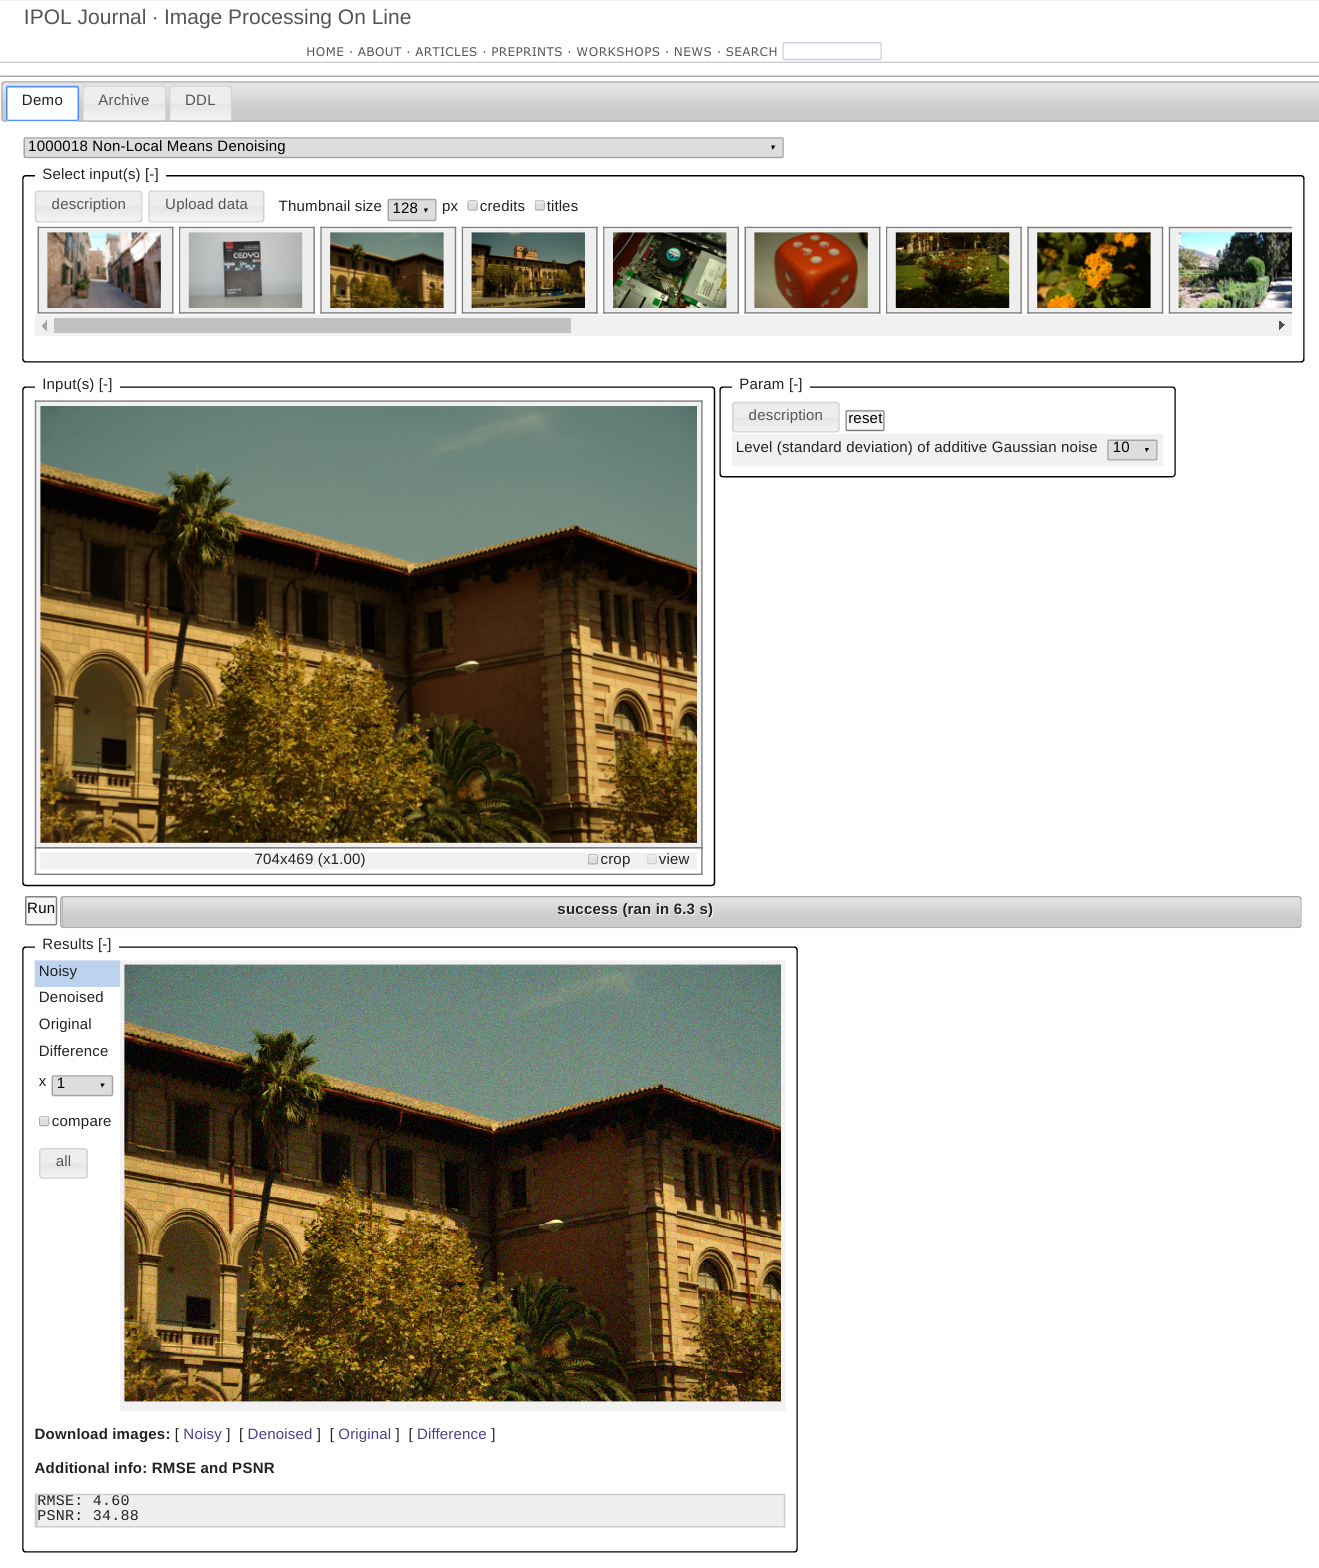
\includegraphics[width=3.5in]{Images/demo_snapshot}
  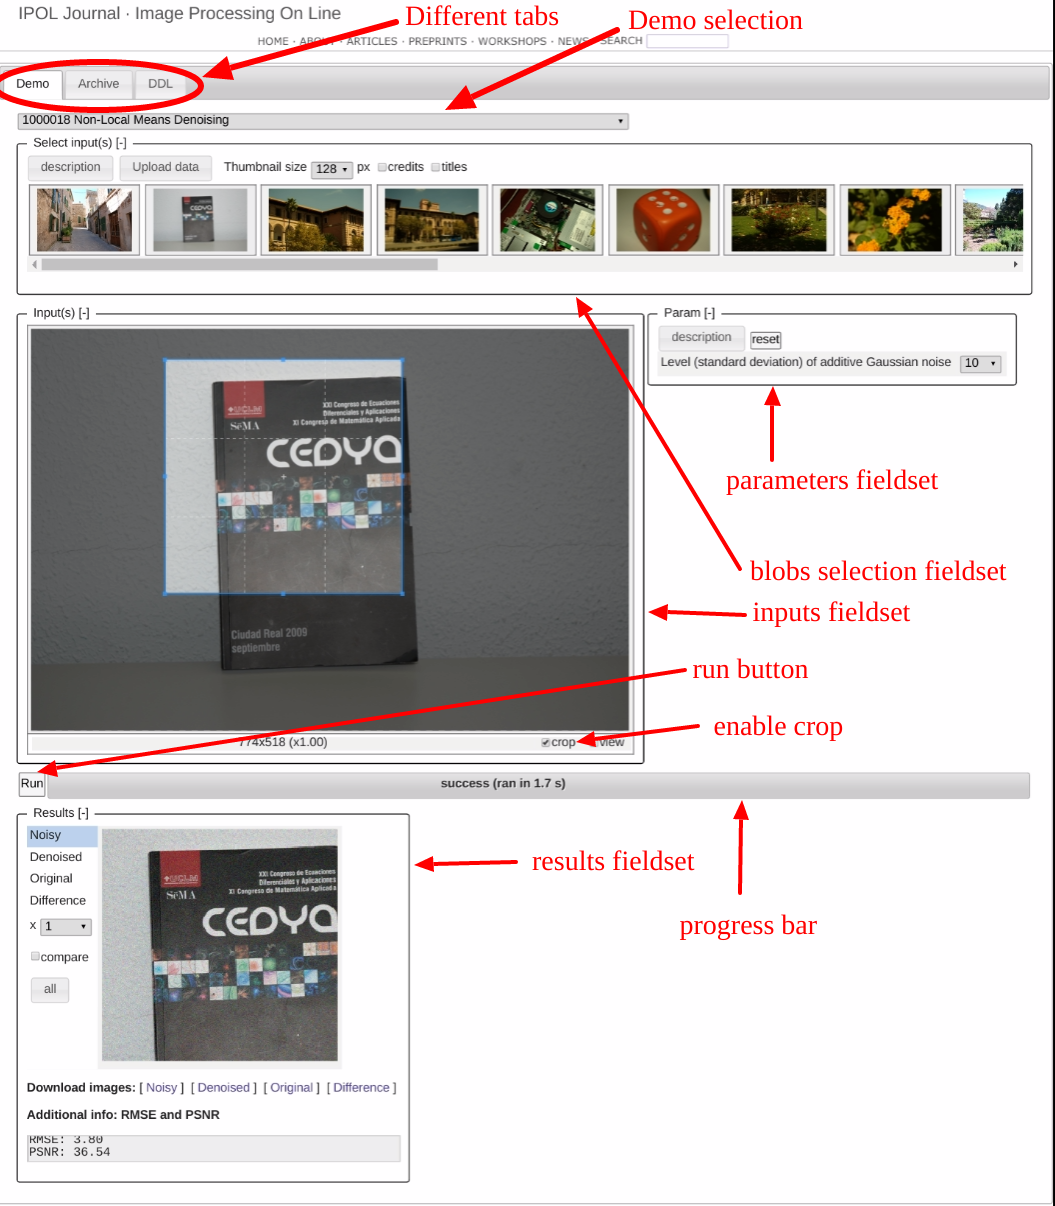
\includegraphics[width=3.5in]{Images/demo_capture}
  \caption{Demo display layout}
  \label{img:demo_snapshot}
\end{figure}

The main flow is as follows:
\begin{itemize}
 \item Step 1: select input demo
    \begin{itemize}
      \item read list of available demos and propose selection,
      \item or read demoid from url params
    \end{itemize}
 \item Step 2: Read and display list of available blobsets 
 \item Step 3: Select input blobset:
    \begin{itemize}
      \item select blobset from the list,
      \item or upload blobset.
    \end{itemize}
 \item Step 4: Display selected blobset 
    \begin{itemize}
      \item if there is a single image, allow crop selection,
      \item if there are several input blobs, show then in an ImageGallery object.
    \end{itemize}
 \item Step 5: Display the parameters and allow their selection. 
 \item Step 6: Allow 'run' button, on run click: 
    \begin{itemize}
      \item display progress bar,
      \item prepare the demo: check for compilation and installation of the source code,
      \item if blobset selection: send input blobset with possible crop,
      \item if blobset upload: crop input (if available) and send input blobset,
      \item execute the demo with the parameters.
    \end{itemize}
 \item Step 7: if upload, send results/parameters to archive. 
 \item Step 8: Display the results.
\end{itemize}

\subsubsection{Page template}

\paragraph{Included scripts and stylesheets}
The file "ipol\_demo.html" contains the page template, where the main displayed components are defined.
The different scripts are included, together with their CSS stylesheets:

\lstinputlisting[language=HTML, , firstnumber=15, firstline=15, lastline=48, 
basicstyle=\scriptsize]{../../ipol_demo/modules/core/static/demo/clientApp/ipol_demo.html}

You will notice the use of the following external modules:
\begin{itemize}
 \item \emph{cropper.js} available at 
        \url{https://github.com/fengyuanchen/cropper} is used to crop input 
        images; 
 \item \emph{noUiSlider} available at 
        \url{http://refreshless.com/nouislider/} is used to create sliders that
        behave better on touch screen. It is combined with wNumb: 
        \url{http://refreshless.com/wnumb/} used to format outputs.
        Only basic features of noUiSlider are used for the moment, but more 
        advanced features could be added in the future, like displaying ticks 
        for example.
  \item In order to upload canvas images, the module 
        \emph{canvas-to-blob} 
        (\url{https://github.com/blueimp/JavaScript-Canvas-to-Blob}) and 
        \emph{blob-util} (\url{https://github.com/nolanlawson/blob-util}) are 
        used.
  \item \emph{sketch.js} is used for drawing mask, it has been 
        modified to better fit the needs of the mask drawing (and also to try 
        to fix a position issue with chrome on touching devices). The original   
        version is available at (\url{http://intridea.github.io/sketch.js/}), 
        the modified version is on the github server of the IPOL demo system.
  \item \emph{history.js} (\url{https://github.com/browserstate/history.js/}) is 
        used to push states on the browser history and to deal with  
        history events.
\end{itemize}

\paragraph{Page tabs} Three tabs are created using jquery ui, the first tab
contains the demo selection, display and execution. The second tab contains
the archive information, and the third tab contains the Demo Description 
Language (DDL) file in JSON format.
\miguel{Are we really copying lines from the source specifying a line range? Of course, we can't do it like that, since obviously if we chage the source code the documentation will desynchronize and won't make sense. Also, you need to explain what the code does, not copying parts of code.}
\lstinputlisting[language=HTML, firstnumber=111,
linerange={111-123}, basicstyle=\scriptsize]{
../../ipol_demo/modules/core/static/demo/clientApp/ipol_demo.html}
$\cdots$
\lstinputlisting[language=HTML, firstnumber=241,
linerange={241-248}, basicstyle=\scriptsize]{
../../ipol_demo/modules/core/static/demo/clientApp/ipol_demo.html}

Additionally, when the user enters the 'Archive' tab, the archive information
is automatically updated and the last archive page is displayed:
\lstinputlisting[language=JavaScript, firstnumber=523,
linerange={523-538}, basicstyle=\scriptsize]{
../../ipol_demo/modules/core/static/demo/clientApp/ipol.js}
To obtain the demo id, we first get the demo list stored within the "demo-select"
HTML element (using the jquery data() function), then we obtain the demo id 
(editordemoid) from the current position of the demo selection widget.

\paragraph{Page fieldsets and other displayed elements}

Four fieldsets are defined in the file ipol\_demo.html: blob selection, inputs, 
parameters and results. It also contains the code to create the progress bar
and the modal dialog to upload data.
The modal dialog is then initialized by the following code:
\lstinputlisting[language=JavaScript, firstnumber=581,
linerange={581-599}, basicstyle=\scriptsize]{
../../ipol_demo/modules/core/static/demo/clientApp/ipol.js}
and the ipol.upload.ManageLocalData() function called by ipol.setDemoPage().

\subsubsection{Step 1: input demo selection}

The list of demos is obtained from the demoinfo module using the service "demo\_list",
in the function ipol.ListDemos(). Once the list is obtained, 
ipol.OnDemoList(demolist) is called.
The demo list is stored in the HTML element "demo-select" and once the demo is
selected (from user selection or from the url parameters), the function 
ipol.setDemoPage() is called.

The function ipol.setDemoPage() first call the service "read\_last\-\_des\-crip\-tion\_from\_demo"
of the "demoinfo" module using ipol.utils.ModuleService():
\lstinputlisting[language=JavaScript, firstnumber=317,
linerange={317-321}, basicstyle=\scriptsize]{
../../ipol_demo/modules/core/static/demo/clientApp/ipol.js}

Once the demo description is returned, it runs the following steps:
\begin{itemize}
  \item empties the contents of the page,
  \item changes its title to contain the demo title,
  \item prepares the webpage to receive the different contents,
  \item displays the parameters if any,
  \item fills the contents of the archive tab,
  \item calls demoinfo module service "get\_blobs\-\_of\-\_demo\-\_by\-\_name\-\_ws"
to get the list of available blobsets for this demo, and calls staticOnDemoBlobs()
method to display them and set their events,
  \item and based on the "origin" parameter:
    \begin{itemize}
      \item if origin is "select\_widget" push a new state to the history,
      \item if origin is "url", if it contains the parameter 'res', displays
            the associated results. If it contains the parameter 'exp', displays
            the corresponding archive experiment.
      \item if origin is "browser\_history", call the callback function "func" 
            given in parameter.
    \end{itemize}
\end{itemize}

\subsubsection{Step 2: read and display list of available blobsets}

The static method ipol.DrawBlobs.staticOnDemoBlobs() returns a function
that creates an instance of ipol.DrawBlobs class, add possible template
to the blob list and displays all the blobs and their associated events.

\subsubsection{Step 3: select input blobset}

The input blobset can be either selected from the proposed list or uploaded from 
local files.
\paragraph{Blobset selection:}
If it is selected by clicking on one of the proposed blobsets, the event will
trigger the creation of a DrawInputs instance with the string "blobset" as origin,
load the input blobset and prepare for running the demo:
\lstinputlisting[language=JavaScript, firstnumber=333,
linerange={333-353}, basicstyle=\scriptsize]{
../../ipol_demo/modules/core/static/demo/clientApp/ipol.drawblobs.js}

\paragraph{Data upload:}

Clicking on the "Upload data" button will display a modal dialog window
where the user can choose the files to upload from his local disk.
\begin{figure}[H]
  \centering
%  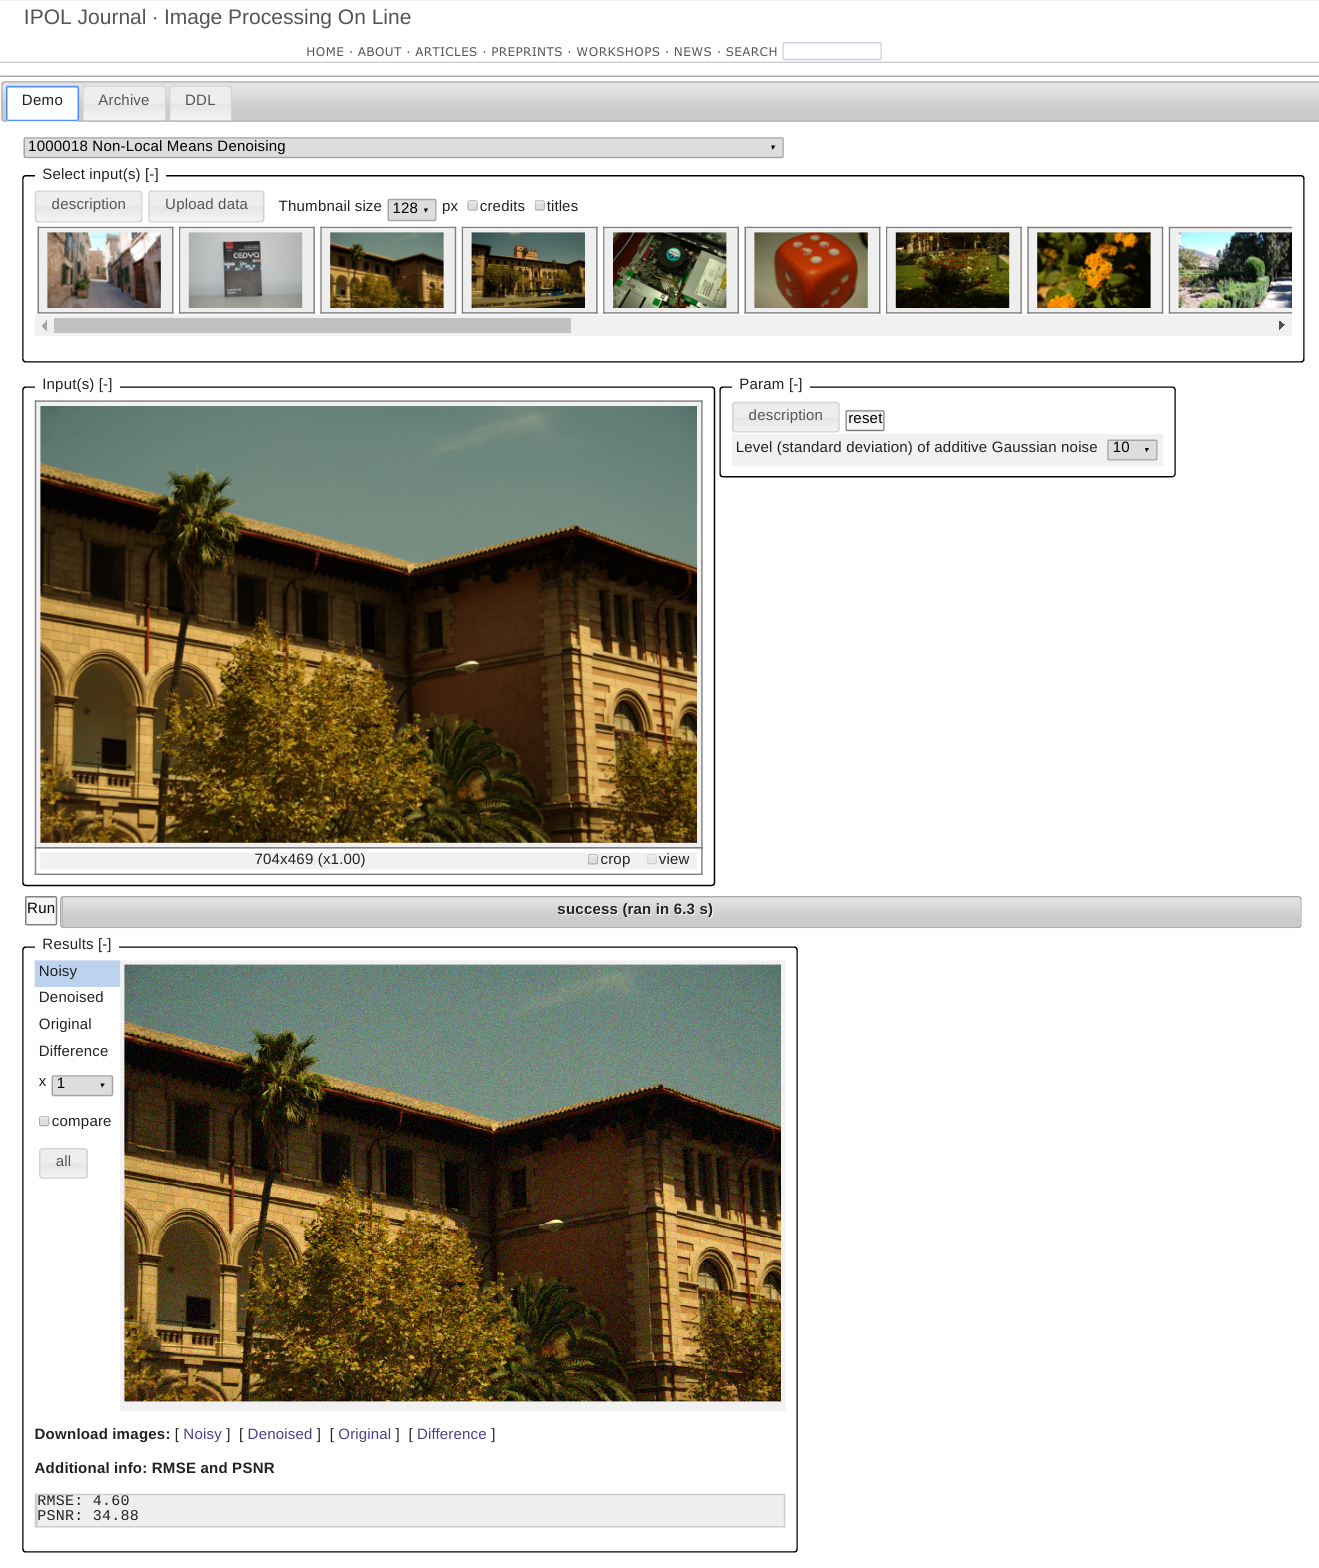
\includegraphics[width=3.5in]{Images/demo_snapshot}
  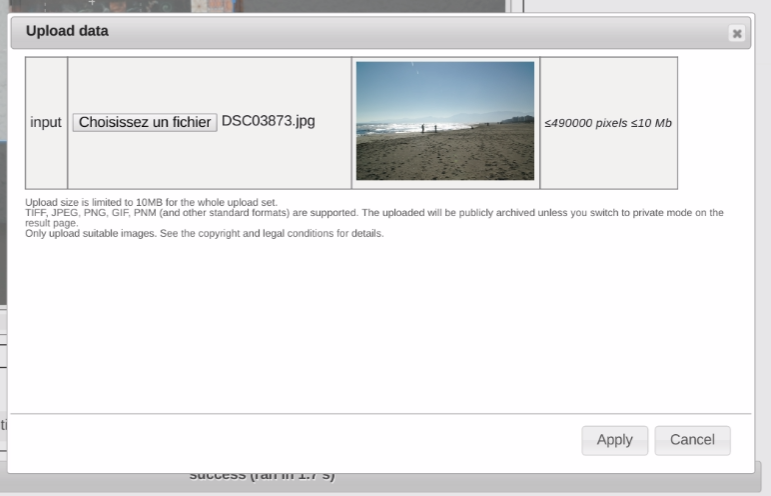
\includegraphics[width=3.5in]{Images/uploadwindow_capture}
  \caption{Upload files modal window}
  \label{img:uploadwindow_snapshot}
\end{figure}

This window is created by the ipol.upload.CreateUploadHTML(), and the function
ipol.upload.UploadBlobsEvents() deals with the file selection and display.
Note that the selected files will only be uploaded to the server before the
demo execution (after clicking on the "run" button).
Once the user accept its selection by clicking on the "Apply" button, 
instances of the DrawInputs and RunDemo classes are created within the 
ipol.upload.ManageLocalData() function:
\lstinputlisting[language=JavaScript, firstnumber=160,
linerange={160-185}, basicstyle=\scriptsize]{
../../ipol_demo/modules/core/static/demo/clientApp/ipol.upload.js}

\subsubsection{Step 4: Display selected blobset}
Once the user has selected a blobset, it is displayed in the inputs fieldset
with its corresponding interface.
The initial HTML code is created by DrawInputs.createHTML() method. 

\paragraph{Single input image}
In the case of a single input image, this input is displayed with a crop option.
The user can crop the input image interactively and also display a zoomed preview
of the crop area on the right. The crop is using the existing "cropper.js" module.

\paragraph{Multiple inputs}
In the case of multiple inputs, the "ImageGallery" class is used to display the 
image representation of each input. In an input is of "image" type, it is its own
image representation. Otherwise, its image representation is a PNG image at the same
position in the blobset, if any.
The image gallery is created by the private method DrawInputs.\_createGallery(inputs\_info).
The "inputs\_info" object contains the titles and contents to be displayed and is created
by the one of the public methods DrawInputs.loadDataFromBlobset() or DrawInputs.loadDataFromLocalFiles().

\paragraph{Inpainting demos}
If the demo DDL has mask drawing enabled (general.drawmask=true), then an drawmask object
of class "ipol.features.Inpainting" is created as a private member \_drawmask of the class
DrawInputs. In this case, the usual displayed input is hidden and the displayed HTML code
contains the result of the function call to \_drawmask.createHTML() that creates all 
the mask drawing interface. The mask image is also added to the hidden ImageGallery object,
it will be updated after each drawing event and it will be used as an image to upload
for the demo execution.

\subsubsection{Step 5: Display the parameters and allow their selection}

The functions related to the display of the parameters are located in the "ipol.drawparams.js"
file and are within the class "ipol.DrawParams". Default parameter values can be reset using
the dedicated button.
The static method ipol.DrawParams.staticUpdateParams() takes care to updating parameters
that may have interdependencies. Currently, only the "visible" properties, and the 
"readonly" type contents are evaluated using javascript eval() function.

\subsubsection{Step 6: deal with 'run' events}

The method "ipol.RunDemo.setRunEvent()" initializes the progress bar and deals
with the click on the "run" button.
The first step is to call the service "demorunner:init\_demo" that checks for the
source code installation and compilation. Once the current demo is successfully
initialized, input data can be either uploaded to defined:
\begin{itemize}
 \item for mask drawing demos, the method \_drawmask.submitDrawMask() is called,
        that will submit the inputs: image and mask.
 \item for non-mask-drawing demos where the input comes from a selected blobset,
        the service "demorunner:input\_select\_and\_crop" is called with all the
        required parameters: demo id, blobset information, crop information.
 \item for non-mask-drawing demos with local files to upload, a local variable
        of type "FormData" is instanciated and filled with the data to upload.
        In the case of a single input image with selected crop, the image
        is reduced to the crop area before its upload (using the getCroppedCanvas
        option of the cropper module). The convertion from canvas or img to 
        blobs that can be uploaded is obtained using either "canvas.toBlob()"
        function or "blobUtil.imgSrcToBlob().then()" function. Once the 
        form data is filled, the private method "\_uploadForm()" is called.
 \item for demos without any input blob, the private method "\_doRun()" is
        called in return of the service "demorunner:init\_noinputs".
\end{itemize}


\subsubsection{Managing browser history}

